\documentclass[12pt]{report}
\usepackage[T1]{fontenc}
\usepackage[utf8]{inputenc}
\usepackage{amsmath,amssymb,amsfonts} % Required for some math elements, equation environment and inline $ (math) $
\usepackage{makeidx}
\usepackage{graphicx} % Required for the inclusion of images
\usepackage{txfonts}
%\usepackage{times} % Uncomment to use the chosen font 
\usepackage[skip=5pt,font={small,it},labelfont=bf]{caption}
\usepackage{subcaption}
\usepackage{siunitx} % Provides the \SI{}{} and \si{} command for typesetting SI units 
\usepackage{color}
\usepackage[english]{babel} %%% SPRAWDZANIE PISOWNI EN
%\usepackage[polish]{babel} %%% SPRAWDZANIE PISOWNI PL

%%% PAGE HEADERS COMMANDS %%%
\usepackage{fancyhdr} % Page Headers and Footers
\pagestyle{fancy} %page style with FancyHDR package
\fancyhf{} % clear the header/footer style
\lhead{\leftmark} % hdr left - standard marking (chapter names)
\rhead{\thepage} % hdr right - page numbering
%\setlength{\textwidth}{14cm}
\setlength{\textheight}{20cm} 

% BIB REF COMMANDS
\usepackage[nottoc,notlot,notlof]{tocbibind}
\usepackage[backend=bibtex,style=alphabetic,sorting=anyvt]{biblatex}  
%Bibliography sorting options
%
%option	description
%nty	sort by name, title, year
%nyt	sort by name, year, title
%nyvt	sort by name, year, volume, title
%anyt	sort by alphabetic label, name, year, title
%anyvt	sort by alphabetic label, name, year, volume, title
%ydtn	sort by year (descending), name, title
%none	entries are processed in citation order
\bibliography{references}

% CODE LISTINGS COMMANDS
\usepackage{verbatim} % Pre-formatted text environment 
\usepackage[linesnumbered,ruled,vlined]{algorithm2e} % Algorithms with ctan algorithm2e 
\usepackage{listings}
\definecolor{mygray}{rgb}{0.4,0.4,0.4}
\definecolor{mygreen}{rgb}{0,0.6,0.4}
\definecolor{myorange}{rgb}{0.8,0.2,0}
\lstset{ 
	basicstyle=\footnotesize\sffamily\color{black},
	keywordstyle=\color{mygreen},
	commentstyle=\color{mygray},
	identifierstyle=\color{blue},
	stringstyle=\color{myorange},
	numbers=left,
	numbersep=5pt,
	numberstyle=\tiny\color{mygray},
	frame=tbTB,
	breakatwhitespace=false,         
	breaklines=true,                 
	captionpos=t,                    
	keepspaces=true, 
	columns=fullflexible,
	showstringspaces=false,
	float=t
	tabsize=2
} 


%\newtheorem{definition}{Definicja} % przykład nowego środowiska 
%\newtheorem{example}{Przykład}[chapter] % przykład nowego środowiska 
%\newtheorem{corollary}{Wniosek}[chapter] % przykład nowego środowiska 

%%% TO DO notes
\usepackage[textsize=footnotesize]{todonotes}
% \usepackage[disable]{todonotes}
\newcommand{\td}[1]{\todo[inline]{TO DO: #1}}

%%% TOC HYPERLINKS %%%
\usepackage{hyperref}
% remember to use \tableofcontents after title
\hypersetup{
	colorlinks,
	citecolor=black,
	filecolor=black,
	linkcolor=black,
	urlcolor=black,
	pdftitle={Generating two-dimensional game maps with use of cellular automata},
	bookmarks=true 
}  

%%% STRONA TYTUŁOWA - DANE
\title{Generating two-dimensional game maps with use of cellular automata}
\author{Michał Wolski}

\begin{document}

\maketitle
\tableofcontents 



%%%%%%%%%%%%%%%%%%%%%%%%%%%%%%
\chapter{Introduction} \label{rozdzial.wstep} 
During recent years, presence of computer games in human lives has increased. The demand for games has shown that playing games, both as a medium of expression and a means for entertainment, is a desirable form of activity. However, as the demand for games rises \footnote{The Interactive Software Federation of Europe compiles and publishes statistics which include frequency of gaming in European countries and show that demand for games is on the rise. \url{https://www.isfe.eu/industry-facts/statistics}} and computer games become increasingly complex, demand for game content must also rise -- game elements such as believable maps, textures, sound and models (among other types of content) are a necessary resource for production of games. Studies such as \autocite{hendrikx2013procedural} show where the evidence for insufficiency of manual content creation may be found. In the study, authors point to work of Kelly and McCabe \autocite{kelly2007citygen}, Lefebvre and Neyret \autocite{lefebvre2003pattern}, Smelik et al. 2009 \autocite{smelik2009survey} and Iosup 2009 \autocite{iosup2009poggi} as sources which reveal game content production as a time-consuming and expensive endeavour.

\subsubsection{Solving the inefficiency issue}
Scientific surveys such as \autocite{hendrikx2013procedural} and \autocite{smelik2009survey} show why investigating procedural generation is useful for the game industry, by providing examples of successful methods which can be used to generate content for games. Primary concerns which drive the interest in automated ways to create game content are the rising project costs and increasing development time.

In order to reduce the cost of game development, allow for greater replay value or provide a feeling of vastness to the game worlds that designers aim to create, procedural content generation techniques can provide an attractive solution to the problem of content creation. Surveys such as \autocite{hendrikx2013procedural}, \autocite{togelius2011search} and \autocite{de2011survey} show what types of game content can be generated and are a good starting point for seeking methods of procedural generation.

\subsubsection{Personal motivation}
During two recent years, the author of this thesis took part in a small, after-hours independent game development project. Working with a group of friends, using Unreal Engine as a tool to develop a simple prototype of a game belonging to the \textit{rogue-like} game genre. The project is still in development phase and finding a good method of map generation can potentially result in contribution of useful features.

%%%%%%%%%%%%%%%
\section{Thesis structure}
The overall structure of this thesis includes introduction followed by three chapters. The second chapter \ref{rozdzial.teoria} serves as a study on possible mechanisms that could be used for procedural generation and specifically, for creation of 2D maps for games. The chapter \ref{rozdzial.praktyka} describes performed experiments, design and implementation of a solution to the problem. Chapter \ref{rozdzial.podsumowanie} summarizes the findings and concludes the thesis, followed by chapter \ref{rozdzial.kod} which lists full source code of the developed solution.

%%%%%%%%%%%%%%%
\section{Objectives}

This work focuses on automated creation of 2-dimensional game maps using a cellular automata approach. We aim to do so by generating small map tiles, which can be later merged into a bigger map. Such approach allows for a degree of control to the map designer - who may want to decide which tiles will be merged and at which locations in the map they will be present. Moreover, we could also allow for editing the tile before placing it in the map. An approach that integrates manual editing or parametrization of desired results with procedural generation techniques has been proposed before \autocite{bidarra2010integrating}, \autocite{smelik2010integrating}, \autocite{smelik2011declarative}.

We focus on creation of maps for games, since literature shows map generation as an interesting area for experimentation, although personal motivation influenced the choice as well.

Beginning experimentation with flat maps on 2-dimensional plane avoids the complexity that may arise when dealing with higher dimensions.

We will investigate existing methods for procedural generation of game maps which resemble cave structures. Then, an approach that may be used for automated creation of such maps will be selected and examined with a focus on implementing a working map generator. Main points of focus for this project are as follows:

\begin{itemize}
	\item research on procedural generation of maps
	\item selecting a promising approach to use
	\item designing a map generator program
	\item implementing the solution in a programming language of choice
\end{itemize}

\td{Objectives - is that all?}

%%%%%%%%%%%%%%%
\section{Thesis scope}

\td{scope - what we will do, what we will not do. specific goals.}

\td{scope - shortly: what could be done instead}




%%%%%%%%%%%%%%%
\section{Technology and tools}

The following paragraphs summarize what tools were involved during the project of thesis preparation and performing the experiments.

\subsection{Hardware} 

All experiments in this thesis have been performed using a laptop with an Intel x64 2.0 \si{GHz} multi-core processor, 16GB RAM and an \textit{nVidia GeForce GTX 560M} graphics card.
 
\subsection{Software} 

Development environment for the purposes of thesis experiments and writing has been set up under Windows 10 operating system with the following software installed:

\begin{itemize}
	\item Visual Studio 2015 Community IDE
	\item CMake for Windows
	\item TeXstudio editor with MikTeX back-end
	\item Git version control system
	\item Notepad++
	\item UMLet open source modelling program
	\item \td{...}
\end{itemize}

Other configuration details include: \td{environment variables, configuration specifics...} 

This thesis has been prepared with \LaTeX\space system for document typesetting.

 
\subsubsection{Programming languages} 

The program that allowed to carry out experiments in this thesis was implemented using the C++ programming language and compiled with MSVC++ 14.0 compiler, natively included in the VS2015 IDE.  

\subsubsection{Libraries} 

The implementation uses following libraries:
\begin{itemize}
	\item Dear ImGui, by Omar Cornut - to easily build an Immediate Mode user interface. Project homepage:  \url{https://github.com/ocornut/imgui}
	\item GLFW 3.2.1 library - to create an OpenGL context and have direct access to texture functions. Project homepage: \url{http://www.glfw.org/}
	\item \td{...} 
\end{itemize}  
 

\subsection{Other tools }
\subsubsection{Design patterns} 
\td{list used design patters, if any. Singleton? Command? Factory?}
 


%%%%%%%%%%%%%%%
\section{Related work (?)} 

\td{think what could be included here}

%%%%%%%%%%%%%%%%%%%%%%%%%%%%%%
\chapter{Research on 2D map generation methods} \label{rozdzial.teoria}

%%%%%%%%%%%%%%%
\section{Definitions} 

Before we start planning a solution to the problem of map generation, we must first define what we mean by maps. As stated in chapter \ref{rozdzial.wstep}, our context does not deal with projections of 3D objects onto a plane, like the fields of geography and cartography do \autocite{snyder1993flattening}. Our goal is simply to generate planar maps. 


\begin{description}
	\item[Map] \todo{what is a map?} 
	\item[Generation] \todo{what generation means?}
\end{description}

\td{2d map types?}

%%%%%%%%%%%%%%%
\section{ Automation - reduction in development time and cost}



\td{ write about PCG in general, short }
\td{ PCG types of content }
\td{ PCG methods }
\td{ focus on maps }





%%%%%%%%%%%%%%%
\section{Existing solutions for 2D map generation}

In scientific surveys on PCG methods, we find approaches to map generation employed in the past. As listed by Hendrikx et al. \autocite{hendrikx2013procedural}, \td{list map procgen methods}

\td{HOW it was done until now? options?}
\td{ ref survey with table of 2d dungeon gen}

\subsection{Cellular automata}

A cellular automaton is a simulation in which every object in a mathematically defined space is being updated at every step of a simulation. Historically, cellular automata and their properties have been studied since the time of first electronic computers \autocite{Sarkar:2000:BHC:349194.349202}. One of the most complete sources on cellular automata is a book summarizing research on CA carried out by Stephen Wolfram since 1980s \autocite{wolfram2002new}, where a classification of cellular automata is shown along with examples for each kind of CA. 

Specifically, 2-dimensional automata operate on a grid of cells with arbitrary discrete dimensions. Each cell in the grid has neighbours, which may be relevant to the simulation rules. Depending on the type of rules which are used by a particular CA, a different type of cell neighbourhood may be used. To present this concept concisely, a short list of definitions follows.

\begin{description}
	\item[Cell] A cell is simply one unit positioned in CA simulation space. Cells have state, which can be simple  - for example, a binary digit, an integer - or more complicated - a real number with constraints, a complex number, or other.  
	\item[Cell neighborhood] In a context of a 2D square grid of cells, neighbourhood is a collection of nearest cells to the selected one.
	\item[Moore's neighbourhood]  Moore neighbourhood includes the cell and its immediate neighbours - one to the north, south, east and west of the cell, as shown in figure \ref{fig:neighborhood_types}.
	\item[Von Neumann neighbourhood] Von Neumann neighbourhood includes 8 closest neighbours of the cell - immediate and diagonal, as shown in figure \ref{fig:neighborhood_types}.
	\item[Other types of neighborhood] It is possible to imagine other types of cell neighbourhoods, possibly including more cell rings around a cell or only a selection of them arranged in a custom pattern. Those cases are beyond the scope of this thesis.
\end{description}
 
\begin{figure}[h]
	\centering
	\begin{subfigure}[b]{0.35\textwidth}
		\centering
		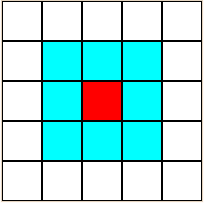
\includegraphics[width=\textwidth]{images/neighborsmoore}
		\caption{Moore neighborhood} 
	\end{subfigure}
	\hfill
	\begin{subfigure}[b]{0.35\textwidth}
		\centering
		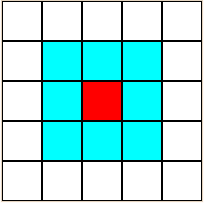
\includegraphics[width=\textwidth]{images/neighborsvonneumann}
		\caption{Von Neumann neighborhood} 
	\end{subfigure} 
	\caption{Two basic types of cell neighborhood}
	\label{fig:neighborhood_types}
\end{figure}


There is a...


\td{}
Every CA simulation also consists of rules which drive the process of cell evolution to its next stage.

\td{ca basics - game of life}
\td{using CA for simulations }
\td{using CA for generation of content}



\subsection{Generative grammars}
\td{What is it? Is relevant to maps? Can we use it? Why?}
\subsection{L-systems} 
\td{What is it? Is relevant to maps? Can we use it? Why?}
\subsection{...}
\td{What is it? Is relevant to maps? Can we use it? Why?}
\subsection{...}
\td{What is it? Is relevant to maps? Can we use it? Why?}

%%%%%%%%%%%%%%%
\section{Choosing a method of generation}

In order to effectively judge the value that a working map generator may bring to a game development project, we need to consider what characteristics should be evaluated. First, a useful generator must be effective at map generation.

\td{how to measure effectiveness? time of map generation, map shape, desirable map features?}

Another point to consider is how easy to use such generator can be. Game designers may ultimately decide to use manual methods of map creation if the method of map generation requires too much effort to include in their project.

\td{how to measure such ease of use? accessibility? }

The third aspect of choice what a generation method could be used is to consider how much value it brings to the designer versus what development costs it can reduce.

\td{how to measure cost?}

The following subsections describe how each of the mentioned aspects can influence the choice of a generation method.

\subsection{Effectiveness} 
\td{study on generation time}
\td{desired characteristics of generated content?}

\subsection{Accessibility} 

\td{study on what makes generation easy to include in game development projects}
\td{integrating manual editing AND procgen}

\subsection{Cost} 
\td{examples of development costs - human resources, machine resources}
\td{which of these costs can be reduced by PCG}




%%%%%%%%%%%%%%%
\section{Chosen approach: cellular automata for 2D map generation}

One of possible proposed approaches is the work of L. Johnson, G. Yannakakis and J. Togelius from IT University of Copenhagen \autocite{johnson2010cellular}. 

Authors describe rules of a cellular automaton which are able to transform a tile filled initially with random distribution of cells into a tile which has interesting properties for a map designer.

\td{authors describe a process - 1 random image 2 apply CA steps as in article cave gen 3 merge tiles, result: maps!} 

\td{short paragraph on the choice of CA for game maps}
\td{why we chose CA for mapgen?}
\td{what are pros and cons of such choice?}

%%%%%%%%%%%%%%%%%%%%%%%%%%%%%%%%%%%%%%%%%%%%%%%%%%%%%%%%%%%%%%%%%%%%%%%%%%%%%%% 
%%%%%%%%%%%%%%%%%%%%%%%%%%%%%%%%%%%%%%%%%%%%%%%%%%%%%%%%%%%%%%%%%%%%%%%%%%%%%%% 
\chapter{Generating and visualizing maps - proposed solution} \label{rozdzial.praktyka} 

\td{describe stages of the project} 




%%%%%%%%%%%%%%%
\section{Analysis of requirements for a map generator}

Having gathered the abstract constructs needed to build a CA map generator in chapter \ref{rozdzial.teoria}, we may proceed to state the requirements formally. 

\subsection{Functional requirements}

First, we must define the desired functions which a useful map generator should provide to the user. 

\begin{itemize}
	\item user interface allowing playing with parameters
	\item rendering each generation step
	\item exporting generated maps
	\item \td{}
\end{itemize}

\subsection{Non-functional requirements}

\begin{itemize}
	\item allow changing parameters by user
	\item format of exported maps must be easy to understand and use
	\item \td{}
\end{itemize}

\subsection{Constraints}

\begin{itemize}
	\item Constraint: time of map tile generation must not exceed 10 seconds.
	\item \td{}
\end{itemize}

%%%%%%%%%%%%%%%
\section{Design}
\subsection{Data structures and persistence}

\td{ how do we store data?}
\td{ diagrams of cell, board}
\td{ exporting data from generator? }
\td{ how designers can get a complete map model? } 

\subsection{Application logic} 

\td{how a generator will work}
\td{behavior diagrams}

\subsection{User interface}

\td{OpenGL immediate mode paradigm}
\td{imgui immediate mode user interface library}

\begin{figure}[h]
	\centering
	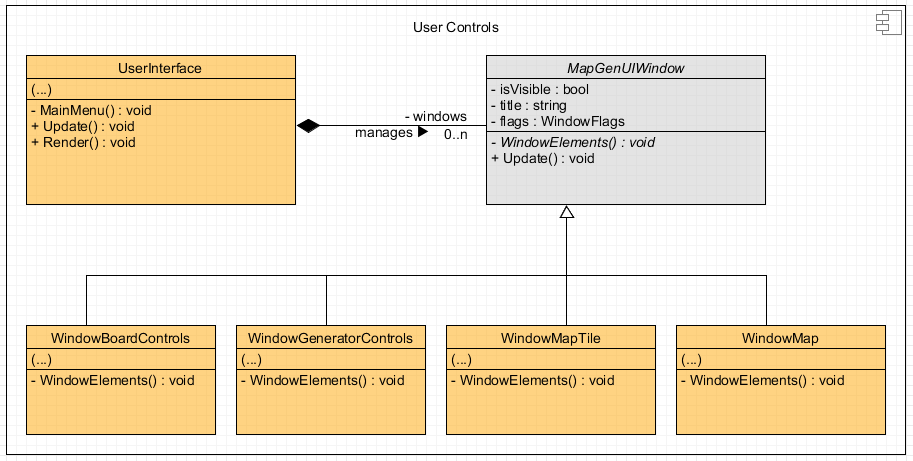
\includegraphics[width=0.8\linewidth]{diagrams/uiwindows}
	\caption[User Interface model]{Example model of classes to be used to construct user interface in the map generator program}
	\label{fig:uiwindows}
\end{figure}

\td{diagram of texture class, used by Component MapGen, uses OpenGL}

\td{mention Bret Victor talks - why we choose Immediate Mode}


%%%%%%%%%%%%%%%
\section{Basic cellular automata simulations}

Having chosen cellular automata as a method for generating maps, we need to have a clear idea about how to approach building a program that could simulate a cellular automaton. One of the helpful resources on the topic of building cellular automata simulations is chapter 7 in Nature of Code, a book by Daniel Shiffman \autocite{shiffman2012nature}, where we can find a short tutorial to build our first CA simulation. There, author describes elementary concepts needed to construct a basic CA, explains how to implement a working simulation and provides helpful exercises. The tutorial is quite useful as a guide, since examples presented in New Kind of Science \autocite{wolfram2002new} are implemented in the Wolfram language and would require familiarity with it. As stated in Nature of Code \autocite{shiffman2012nature}, a 2-dimensional CA would need the following key elements to be simulated:

\begin{itemize}
	\item Cell state - every cell has a state updated on each simulation step,
	\item Grid - a space on which cells are placed,
	\item Neighbourhood - each cell needs to know the state of its neighbours to update its state.
\end{itemize}

In order to represent the cells of an automaton, a primitive data type is sufficient. However, we could design a class which will act as a collection of cells and provide additional utility to the user. Figure \ref{fig:boardcell} presents an example model of a class that would encapsulate a collection of cell states while also preserving information about the board on which those cells are placed. 

\begin{figure}[h]
	\centering
	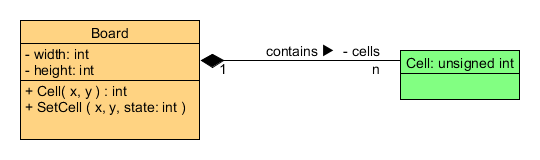
\includegraphics[width=0.8\linewidth]{diagrams/boardcell01}
	\caption{ A possible model of a Board Class which holds cell states in its block of memory and lets its user change their states} 
	\label{fig:boardcell}
\end{figure}

We can also assign a number to each cell \td{why?} as shown in table \ref{tab:cellneighbors}.

\begin{table}[h]
	\centering
	\begin{tabular}{| l | l | l |}
		\hline 
		0 & 1 & 2 \\
		\hline
		7 & S & 3 \\
		\hline
		6 & 5 & 4 \\ 
		\hline
	\end{tabular}
	\caption{Cell neighbours, numbered. \textit{S} denotes selected cell. Cells marked with odd numbers are members of Moore neighborhood of selected cell and all numbered cells are members of Von Neumann neighbourhood of it. }
	\label{tab:cellneighbors}
\end{table}


Such abstraction creates an easy to use interface for further development and is also sufficient to access the values of neighbors to the selected cell. However, in some CA simulations summing the values of cells in neighbourhood is a common operation, so we can include variations of it for convenience. Similarly, a method to translate cell states into texture points would be welcome, since we may possibly need a way to display the state of CA board on screen. Adding those elements to our abstraction yields a class presented on figure \ref{fig:boardcell2}.
 
 \begin{figure}[h]
 	\centering
 	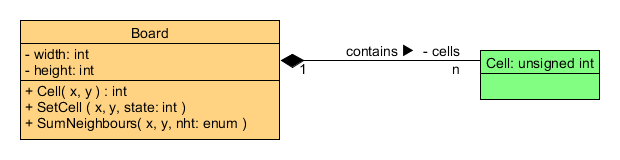
\includegraphics[width=0.8\linewidth]{diagrams/boardcell02}
 	\caption{ Revised Board abstraction - added methods for neighbor sums and translation of cell states to texels} 
 	\label{fig:boardcell2}
 \end{figure}

\td{add neighbor methods to board2}
\td{result of what it all does?}

At this point, we could also observe a common property of cellular automata  - whenever cell states need to change (the simulation moves to a later step), the state change is applied to every cell in the grid before simulation step ends \autocite{wolfram1984cellular} and cells do not need to be updated in sequence if only all cells will be changed before the next step. Hence, cell state updates could be applied in parallel to reduce the time needed to compute the simulation step. One way to do so would be to apply the findings presented by Reno Fourie in his thesis about applying CUDA technology to reduce time to compute next state of the board in case of 2-dimensional cellular automata \autocite{fourie2015parallel}.

\td{what else to include?}
\td{more on CA, 2dim CA?}


%%%%%%%%%%%%%%%
\section{Generating maps with CA}

Since the goal of this work is not to just implement a working cellular automaton simulation, we need to find a way to generate maps using CA simulation. 

\begin{figure}[h]
	\centering
	\begin{subfigure}[b]{0.2\textwidth}
		\centering
		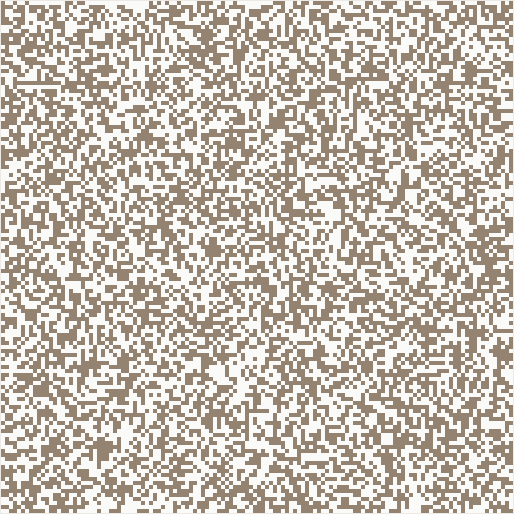
\includegraphics[width=\textwidth]{images/step1}
		\caption{Step 1 - random noise} 
	\end{subfigure}
	\hfill
	\begin{subfigure}[b]{0.2\textwidth}
		\centering
		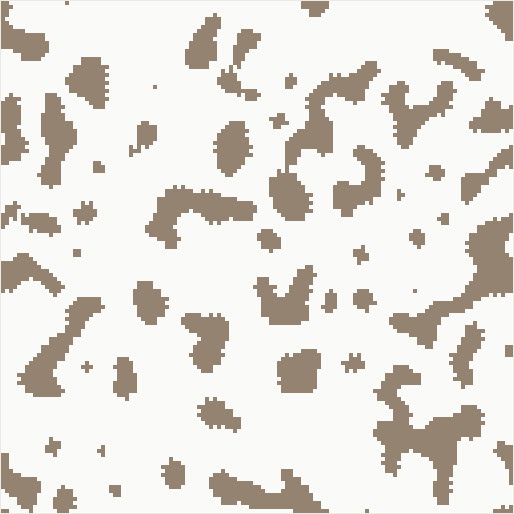
\includegraphics[width=\textwidth]{images/step2}
		\caption{Step 2 - generated tile} 
	\end{subfigure}
	\hfill
	\begin{subfigure}[b]{0.2\textwidth}
		\centering
		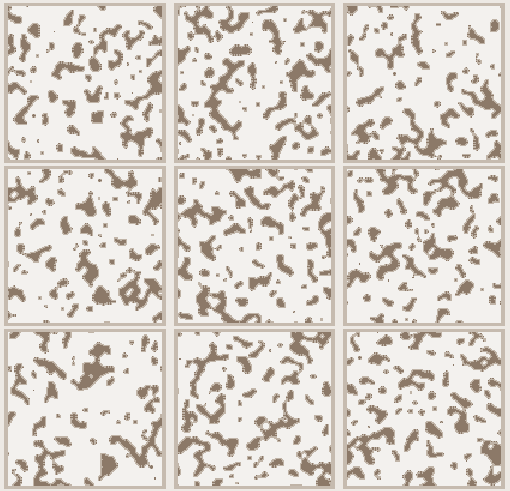
\includegraphics[width=\textwidth]{images/step3}
		\caption{Step 3 - tiles in a grid} 
	\end{subfigure}
	\hfill
	\begin{subfigure}[b]{0.2\textwidth}
		\centering
		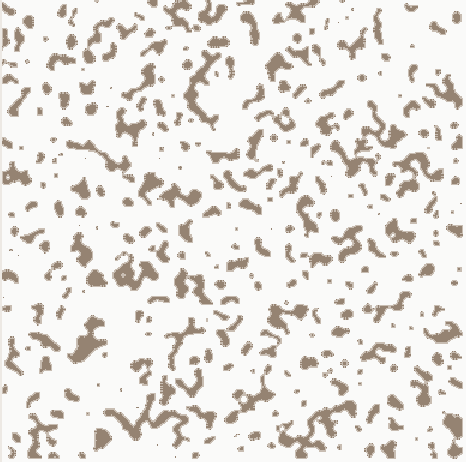
\includegraphics[width=\textwidth]{images/step4}
		\caption{Step 4 - complete map} 
	\end{subfigure}
	\caption{Four stages of map construction}
	\label{fig:map_steps}
\end{figure}






%%%%%%%%%%%%%%%
\section{Implementation}

\td{describe how it all works now, with object diagrams}
\td{refer to code itself}


%%%%%%%%%%%%%%%
\section{Tests} 

\subsection{Performance test}

%%%%%%%%%%%%%%%
\section{Deployment (?)} 

%%%%%%%%%%%%%%%%%%%%%%%%%%%%%%
\chapter{Conclusions} \label{rozdzial.podsumowanie}

%%%%%%%%%%%%%%%
\section{Evaluation of results} 

\subsection{Effectiveness}
\subsection{Accessibility}
\subsection{Cost}

%%%%%%%%%%%%%%%
\section{Perspectives for usage }

\td{map generator will be used in game project codenamed 'UW'}

%%%%%%%%%%%%%%%
\section{Further work}

 
%%%%%%%%%%%%%%%%%%%%%%%%%%%%%%
\chapter{Full source code} \label{rozdzial.kod} 
% use firstline=1, lastline=200 to load a snippet from file instead of all lines
\lstinputlisting[language=C++, caption=main.cpp Source Code]{../main.cpp}
\lstinputlisting[language=C++, caption=Board.h Source Code]{../Board.h}
\lstinputlisting[language=C++, caption=Map.h Source Code]{../Map.h}
\lstinputlisting[language=C++, caption=Ruleset.h Source Code]{../Ruleset.h}
\lstinputlisting[language=C++, caption=TextureAtlas.h Source Code]{../TextureAtlas.h}
\lstinputlisting[language=C++, caption=TileGenerator.h Source Code]{../TileGenerator.h}
\lstinputlisting[language=C++, caption=UserInterface\_MapGenerator.h Source Code]{../UserInterface_MapGenerator.h}
\lstinputlisting[language=C++, caption=Window\_Base.h Source Code]{../Window_Base.h}
\lstinputlisting[language=C++, caption=WindowBoardControls.h Source Code]{../WindowBoardControls.h}
\lstinputlisting[language=C++, caption=WindowBoardImage.h Source Code]{../WindowBoardImage.h}
\lstinputlisting[language=C++, caption=WindowGeneratorControls.h Source Code]{../WindowGeneratorControls.h}
\lstinputlisting[language=C++, caption=WindowMapTileGrid.h Source Code]{../WindowMapTileGrid.h}

%%%%%%%%%%%%%%%%%%%%%%%%%%%%%%
%%% KONIEC PRACY %%%%%%%%%%%%%
%%%%%%%%%%%%%%%%%%%%%%%%%%%%%%
\printbibliography[heading=bibintoc]

\addcontentsline{toc}{chapter}{List of figures} 
\listoffigures

\addcontentsline{toc}{chapter}{List of tables} 
\listoftables

\addcontentsline{toc}{chapter}{List of abbreviations and acronyms} 
%%%%%%%%%%%%%%%
\chapter*{List of abbreviations and acronyms} 

The following terms, abbreviations and acronyms have been used in the thesis.

\begin{description}
	\item[CA] Cellular Automaton. A simulation consisting of cell objects.
	\item[PCG] Procedural Content Generation. An automated process of creation.   
\end{description}
\td{(?)}  

\addcontentsline{toc}{chapter}{Attachments} 
%%%%%%%%%%%%%%%%%%%%%%%%%%%%%%
\chapter*{Attachments}
\begin{enumerate}
\item List of To Do Notes \todo{list of todos - remove this before submitting thesis} 
\item \td{include thesis defence documents}
\item \td{?}
\item \td{?}
\item \td{?}
\end{enumerate}

\listoftodos

\end{document}
